% ============================================================
%  NEORV32 Accelerator for Cryptography
%  Ascon-AEAD128 Hardware Accelerator
%  Design Document
%  Author: Mohammadi Masoudi Ramin
%  Style matched to the RASD (Rev. 0.5)
% ============================================================
\documentclass[11pt,a4paper]{article}

\usepackage[T1]{fontenc}
\usepackage[utf8]{inputenc}
\usepackage[margin=2.5cm]{geometry}
\usepackage{hyperref}
\usepackage{booktabs}
\usepackage{longtable}
\usepackage{array}
\usepackage{xcolor}
\usepackage{colortbl}
\usepackage{listings}
\usepackage{tikz}
\usetikzlibrary{arrows.meta,positioning,shapes.geometric,shapes.misc,calc,fit,automata,backgrounds}
\usepackage{amsmath}
\usepackage{amssymb}
\usepackage{graphicx}
\usepackage{fancyhdr}
\usepackage{titlesec}
\usepackage{enumitem}
\usepackage{float}
\usepackage{multirow}
\usepackage{tabularx}
\usepackage{tcolorbox}
\tcbuselibrary{skins,breakable}

% -- Colours ---------------------------------------------------
\definecolor{docblue}{RGB}{0,51,102}
\definecolor{doclblue}{RGB}{0,85,128}
\definecolor{reqbg}{RGB}{235,244,255}
\definecolor{reqframe}{RGB}{70,100,150}
\definecolor{nfrbg}{RGB}{240,255,240}
\definecolor{nfrframe}{RGB}{40,120,70}
\definecolor{codebg}{RGB}{247,247,247}
\definecolor{tabhead}{RGB}{0,51,102}
\definecolor{rowalt}{RGB}{243,247,255}
\definecolor{warnbg}{RGB}{255,251,230}
\definecolor{warnframe}{RGB}{170,120,0}
\definecolor{stateblue}{RGB}{0,70,140}
\definecolor{statefill}{RGB}{220,232,250}
\definecolor{hwfill}{RGB}{225,238,252}
\definecolor{swfill}{RGB}{234,245,234}

\hypersetup{
  colorlinks=true, linkcolor=docblue, urlcolor=doclblue, citecolor=docblue,
  pdftitle={NEORV32 Ascon-AEAD128 Hardware Accelerator: Design Document},
  pdfauthor={Mohammadi Masoudi Ramin}
}

\titleformat{\section}
  {\Large\bfseries\color{docblue}}{\thesection}{1em}{}
  [\color{docblue}\rule{\linewidth}{0.6pt}]
\titleformat{\subsection}
  {\large\bfseries\color{docblue}}{\thesubsection}{1em}{}
\titleformat{\subsubsection}
  {\normalsize\bfseries\color{doclblue}}{\thesubsubsection}{1em}{}

\pagestyle{fancy}\fancyhf{}
\fancyhead[L]{\small\color{docblue}\textbf{NEORV32 Ascon-AEAD128 Hardware Accelerator}}
\fancyhead[R]{\small\color{docblue}Design Document}
\fancyfoot[C]{\small\thepage}
\renewcommand{\headrulewidth}{0.4pt}

\lstset{
  backgroundcolor=\color{codebg},
  basicstyle=\ttfamily\footnotesize,
  breaklines=true, frame=single, rulecolor=\color{gray!35},
  numbers=left, numberstyle=\tiny\color{gray!55},
  keywordstyle=\color{docblue}\bfseries,
  commentstyle=\color{gray!65}\itshape,
  stringstyle=\color{doclblue},
  xleftmargin=2em, framexleftmargin=2em,
  aboveskip=8pt, belowskip=6pt
}

\newcommand{\warn}[1]{%
  \begin{tcolorbox}[
    enhanced, colback=warnbg, colframe=warnframe,
    arc=2pt, boxrule=0.5pt, left=6pt, right=6pt, top=3pt, bottom=3pt,
    before upper={\small}]
  \textbf{\color{warnframe}Note:} #1
  \end{tcolorbox}\vspace{3pt}}

\newcommand{\choice}[2]{%
  \begin{tcolorbox}[
    enhanced, colback=reqbg, colframe=reqframe,
    arc=2pt, boxrule=0.5pt, left=6pt, right=6pt, top=3pt, bottom=3pt,
    attach boxed title to top left={yshift=-2mm, xshift=8pt},
    boxed title style={colback=reqframe, arc=2pt, boxrule=0pt,
                       left=4pt, right=4pt, top=2pt, bottom=2pt},
    title={\small\bfseries\color{white}Design choice\enspace\textbar\enspace\textit{#1}},
    before upper={\small}]
  #2
  \end{tcolorbox}\vspace{3pt}}

\newcolumntype{L}[1]{>{\raggedright\arraybackslash}p{#1}}
\newcolumntype{C}[1]{>{\centering\arraybackslash}p{#1}}
\newcommand{\thd}[1]{\cellcolor{tabhead}\color{white}\textbf{\small #1}}
\newcommand{\trow}{\rowcolor{rowalt}}
\newcommand{\code}[1]{\texttt{\small #1}}

\setlength{\parskip}{5pt}
\setlength{\parindent}{0pt}
\setlist[itemize]{noitemsep, topsep=2pt}
\setlist[enumerate]{noitemsep, topsep=2pt}

% ============================================================
\begin{document}
% ============================================================

\begin{titlepage}
\centering
\vspace*{2.5cm}
{\color{docblue}\rule{\linewidth}{1.2pt}}\\[0.6cm]
{\Huge\bfseries\color{docblue} NEORV32 Ascon-AEAD128\\[0.2cm] Hardware Accelerator}\\[0.4cm]
{\LARGE\color{doclblue} Design Document}\\[0.3cm]
{\color{docblue}\rule{\linewidth}{1.2pt}}\\[1.2cm]
{\large A tiered, model-driven Ascon (NIST SP 800-232) accelerator,\\
integrated as an XBUS peripheral on a fully-open RISC-V SoC\\
and validated on silicon.}\\[2cm]
{\large\textbf{Mohammadi Masoudi Ramin}}\\[0.3cm]
{\normalsize Politecnico di Milano}\\[0.3cm]
{\normalsize Companion to the Requirements \& Design Document (RASD)}\\
\vfill
{\small This document describes the \emph{as-built} design and reflects the
state validated on a Tang Nano 20K.}
\end{titlepage}

\tableofcontents
\newpage

% ------------------------------------------------------------
\section{Purpose and Scope}
This document describes the design of the Ascon-AEAD128 hardware accelerator and
its integration into a RISC-V system-on-chip. It is a companion to the RASD: the
RASD states \emph{what} the system must do; this document states \emph{how} it is
built and \emph{why} each structural choice was made. It reflects the design as
actually realised and validated on hardware, not an idealised plan.

The scope covers: the generator and golden model that produce the RTL; the
accelerator datapath and its five-layer module hierarchy; the register-level
programming interface; the SoC integration over NEORV32's external bus (XBUS);
the fully-open build toolchain; and the four-layer verification strategy. The
measured on-silicon results are reported separately in the Project Report.

% ------------------------------------------------------------
\section{System Overview}

\subsection{What the system is}
The system is a cryptographic co-processor for authenticated encryption. A RISC-V
CPU (NEORV32) runs application firmware; when it needs Ascon-AEAD128 encryption or
decryption, it hands the key, nonce, associated data and payload to a dedicated
hardware block over a memory-mapped interface, and reads back the ciphertext and
authentication tag. The accelerator performs the Ascon permutation in hardware,
which is far faster than computing it in software on the same small core.

The complete signal path, from the abstract specification down to the programmed
FPGA, is:

\begin{center}
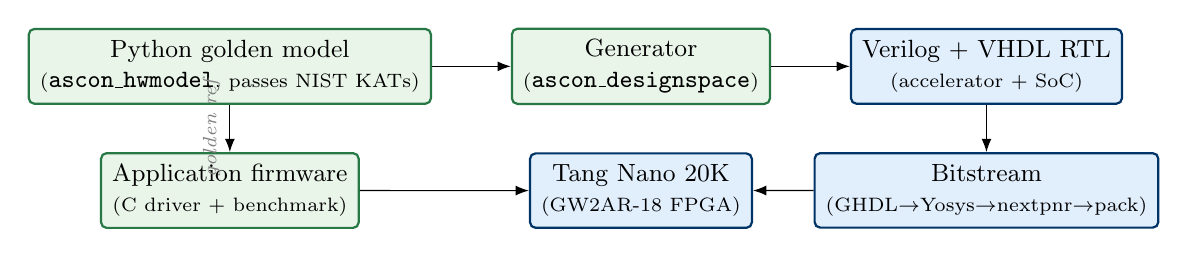
\begin{tikzpicture}[
  node distance=6mm and 10mm, >=Latex,
  box/.style={draw=docblue, thick, rounded corners=2pt, fill=statefill,
              align=center, minimum height=8mm, inner sep=4pt, font=\small},
  swb/.style={box, fill=swfill, draw=nfrframe},
  hwb/.style={box, fill=hwfill},
  lbl/.style={font=\scriptsize\itshape, color=gray}]
\node[swb] (model) {Python golden model\\\scriptsize(\code{ascon\_hwmodel}, passes NIST KATs)};
\node[swb, right=of model] (gen) {Generator\\\scriptsize(\code{ascon\_designspace})};
\node[hwb, right=of gen] (rtl) {Verilog + VHDL RTL\\\scriptsize(accelerator + SoC)};
\node[hwb, below=of rtl] (bit) {Bitstream\\\scriptsize(GHDL$\to$Yosys$\to$nextpnr$\to$pack)};
\node[hwb, below=of gen] (fpga) {Tang Nano 20K\\\scriptsize(GW2AR-18 FPGA)};
\node[swb, below=of model] (fw) {Application firmware\\\scriptsize(C driver + benchmark)};
\draw[->] (model) -- (gen);
\draw[->] (gen) -- (rtl);
\draw[->] (rtl) -- (bit);
\draw[->] (bit) -- (fpga);
\draw[->] (fw) -- (fpga);
\draw[->] (model) -- (fw) node[midway,lbl,rotate=90,anchor=south]{golden ref};
\end{tikzpicture}
\end{center}

\subsection{Integrated block diagram}
Inside the SoC, the accelerator is one peripheral among several, reached through
the bus infrastructure of the NEORV32 core.

\begin{center}
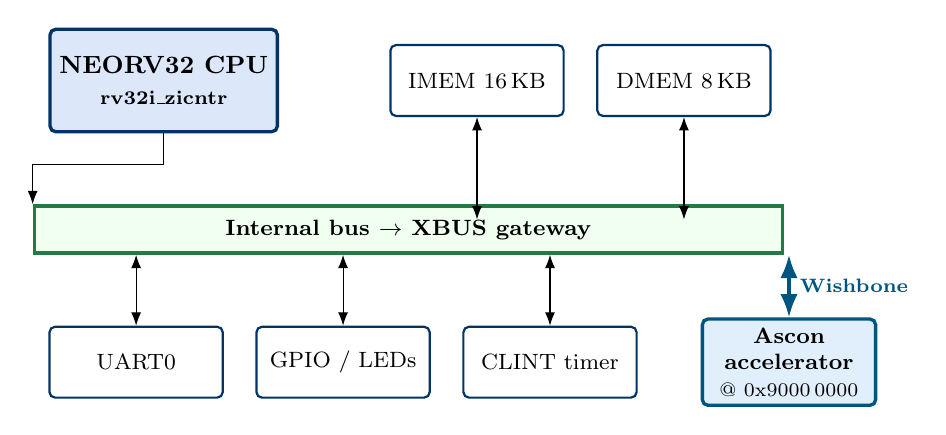
\begin{tikzpicture}[
  >=Latex, node distance=5mm,
  cpu/.style={draw=docblue, very thick, rounded corners=2pt, fill=statefill,
              align=center, minimum width=26mm, minimum height=13mm, font=\small\bfseries},
  per/.style={draw=docblue, thick, rounded corners=2pt, fill=white,
              align=center, minimum width=22mm, minimum height=9mm, font=\footnotesize},
  acc/.style={per, fill=hwfill, draw=doclblue, very thick},
  bus/.style={draw=nfrframe, very thick, fill=nfrbg, minimum width=95mm,
              minimum height=6mm, font=\footnotesize\bfseries}]
\node[cpu] (cpu) {NEORV32 CPU\\\scriptsize rv32i\_zicntr};
\node[per, right=14mm of cpu] (imem) {IMEM 16\,KB};
\node[per, right=4mm of imem] (dmem) {DMEM 8\,KB};
\node[bus, below=9mm of cpu.south west, anchor=north west, xshift=-2mm] (bus) {Internal bus $\to$ XBUS gateway};
\node[per, below=9mm of bus.south west, anchor=north west, xshift=2mm] (uart) {UART0};
\node[per, right=4mm of uart] (gpio) {GPIO / LEDs};
\node[per, right=4mm of gpio] (clint) {CLINT timer};
\node[acc, right=8mm of clint] (acc) {\textbf{Ascon}\\\textbf{accelerator}\\\scriptsize @ 0x9000\,0000};
\draw[->] (cpu.south) -- ++(0,-4mm) -| (bus.north west) node[pos=0.25,above,font=\scriptsize]{};
\draw[<->] (imem.south) -- ++(0,-13mm);
\draw[<->] (dmem.south) -- ++(0,-13mm);
\draw[<->] (bus.south -| uart.north) -- (uart.north);
\draw[<->] (bus.south -| gpio.north) -- (gpio.north);
\draw[<->] (bus.south -| clint.north) -- (clint.north);
\draw[<->, doclblue, very thick] (bus.south -| acc.north) -- (acc.north)
      node[midway,right,font=\scriptsize\bfseries,color=doclblue]{Wishbone};
\end{tikzpicture}
\end{center}

The accelerator is deliberately \emph{loosely coupled}: it is a bus peripheral,
not a change to the CPU pipeline or instruction set. Any address the CPU issues
that is not claimed by internal memory or the I/O region is routed by NEORV32's
bus gateway to the external bus (XBUS), where the accelerator lives.

% ------------------------------------------------------------
\section{The Generator and Golden Model}

\subsection{Model-first methodology}
The design is not written directly in RTL. The single source of truth is a typed
Python model of Ascon (\code{ascon\_hwmodel}) that implements the NIST SP 800-232
permutation and AEAD128 mode and passes the official Known-Answer Tests. From this
model, a generator (\code{ascon\_designspace}) emits the Verilog datapath and the
constants (round constants, IV, S-box) as generated headers. The RTL and the
golden reference therefore share one definition of ``correct.''

\choice{Golden-model-first over hand-written RTL}{%
A validated executable specification is generated \emph{into} the RTL and reused
as the checking oracle. This removes the most common source of crypto-hardware
bugs --- a subtle divergence between the implementation and the specification ---
because both are derived from the same model. It also makes the design
parameterisable: the model describes a family of configurations, and the
generator realises a chosen point.}

\subsection{Configuration space}
The model captures a design space along several architectural axes (permutation
unrolling, datapath width, interface style, buffering), of which one point is
realised here. The realised point is chosen for the constraints of a small FPGA:
a single-round-per-cycle permutation, a 64-bit-word datapath, an AXI-Stream front
end wrapped for memory-mapped access, and bounded on-chip payload buffers.

% ------------------------------------------------------------
\section{Accelerator Architecture}

\subsection{Module hierarchy}
The accelerator is built as five nested layers, each with a single
responsibility and each verified against the model in isolation. From the crypto
core outward:

\begin{center}
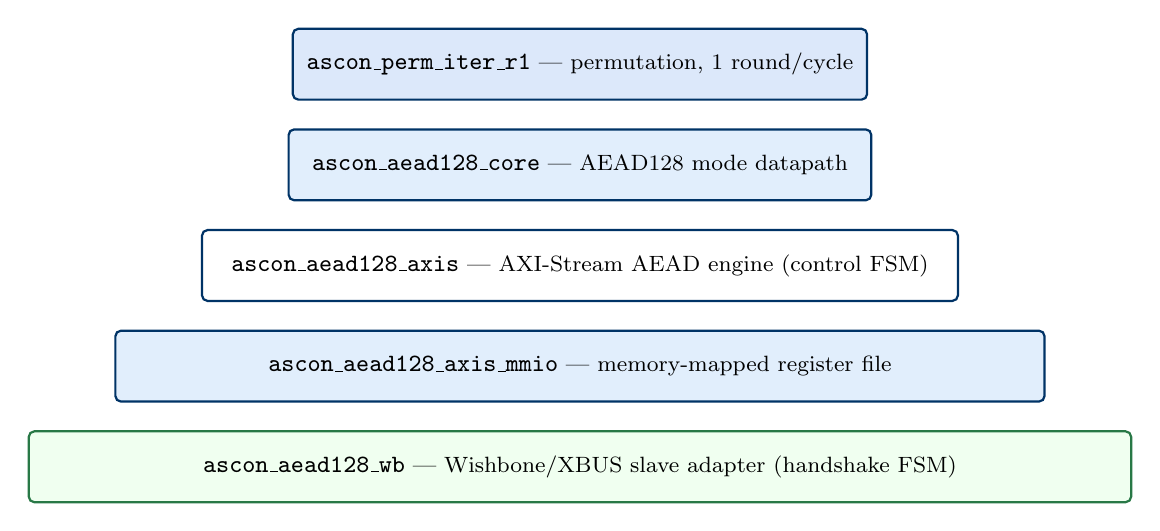
\begin{tikzpicture}[
  >=Latex, node distance=3.5mm,
  lyr/.style={draw=docblue, thick, rounded corners=2pt, align=center,
              minimum height=9mm, font=\footnotesize, inner sep=5pt},
  L1/.style={lyr, fill=statefill, minimum width=52mm},
  L2/.style={lyr, fill=hwfill, minimum width=74mm},
  L3/.style={lyr, fill=white, minimum width=96mm},
  L4/.style={lyr, fill=hwfill, minimum width=118mm},
  L5/.style={lyr, fill=nfrbg, draw=nfrframe, minimum width=140mm},
  note/.style={font=\scriptsize\itshape, color=gray, anchor=west}]
\node[L5] (wb) {\code{ascon\_aead128\_wb} --- Wishbone/XBUS slave adapter (handshake FSM)};
\node[L4, above=of wb] (mmio) {\code{ascon\_aead128\_axis\_mmio} --- memory-mapped register file};
\node[L3, above=of mmio] (axis) {\code{ascon\_aead128\_axis} --- AXI-Stream AEAD engine (control FSM)};
\node[L2, above=of axis] (core) {\code{ascon\_aead128\_core} --- AEAD128 mode datapath};
\node[L1, above=of core] (perm) {\code{ascon\_perm\_iter\_r1} --- permutation, 1 round/cycle};
\end{tikzpicture}
\end{center}

\begin{itemize}
\item \textbf{Permutation} --- one Ascon round per clock (add round constant,
      substitution layer, linear diffusion). The smallest permutation variant;
      it is the crypto primitive shared by every AEAD phase.
\item \textbf{AEAD128 core} --- sequences the mode: initialise from key and nonce,
      absorb associated data, process the message, finalise and emit the tag,
      invoking the permutation the correct number of times per phase.
\item \textbf{AXI-Stream engine} --- a control FSM that receives the payload as a
      stream (associated data then message, distinguished by a sideband bit),
      drives the core, and emits the output stream. Its ready signal is asserted
      only while it is in its receive state.
\item \textbf{MMIO register file} --- exposes the driver-visible registers
      (control, status, key, nonce, lengths, data-in, data-out, tag, cycle count,
      error code) and bridges register writes/reads to the stream engine.
\item \textbf{Wishbone adapter} --- presents a Wishbone-b4 slave to NEORV32's
      XBUS and translates its pulsed-strobe handshake to the register file.
\end{itemize}

\subsection{Engine control FSM}
The stream engine's states and transitions:

\begin{center}
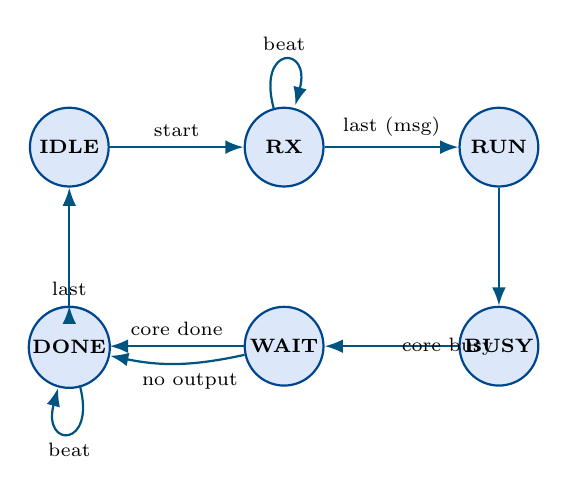
\begin{tikzpicture}[
  >=Latex, node distance=15mm and 17mm,
  st/.style={draw=stateblue, thick, circle, fill=statefill, minimum size=10mm,
             font=\scriptsize\bfseries, inner sep=1pt},
  every edge/.style={draw=doclblue, thick, ->}, font=\scriptsize]
\node[st] (idle) {IDLE};
\node[st, right=of idle] (rx) {RX};
\node[st, right=of rx] (run) {RUN};
\node[st, below=of run] (busy) {BUSY};
\node[st, left=of busy] (wait) {WAIT};
\node[st, left=of wait] (tx) {TX};
\node[st, below=of idle] (done) {DONE};
\path (idle) edge node[above]{start} (rx);
\path (rx) edge[loop above] node{beat} (rx);
\path (rx) edge node[above]{last (msg)} (run);
\path (run) edge (busy);
\path (busy) edge node[right]{core busy} (wait);
\path (wait) edge node[above]{core done} (tx);
\path (tx) edge[loop below] node{beat} (tx);
\path (wait) edge[bend left=12] node[below,pos=0.4]{no output} (done);
\path (tx) edge node[above]{last} (done);
\path (done) edge node[left]{} (idle);
\end{tikzpicture}
\end{center}

\warn{The engine is \emph{start-first}: it asserts stream-ready only after leaving
IDLE (i.e.\ after \code{START}). Driving payload beats before starting the engine
stalls forever. This single fact dictated both the driver's write ordering and the
programming sequence in Section~\ref{sec:prog}.}

% ------------------------------------------------------------
\section{Programming Interface}
\label{sec:prog}

\subsection{Register map}
The accelerator occupies a small window on XBUS. Byte offsets from the base
address (\code{0x9000\,0000}):

\renewcommand{\arraystretch}{1.25}
\begin{center}
\begin{tabular}{L{2.1cm} L{2.4cm} L{9.6cm}}
\thd{Offset} & \thd{Register} & \thd{Purpose}\\
\trow \code{0x00} & CONTROL & \code{START} (bit 0), \code{DECRYPT} (bit 1), \code{CLEAR} (bit 8)\\
\code{0x04} & STATUS & done, error, input-ready, output-valid flags\\
\trow \code{0x08} & MODE & AEAD variant selector\\
\code{0x0C} & CAPABILITIES & feature bits: AEAD128, cycle counter, stream data\\
\trow \code{0x10}/\code{0x14} & AD\_LEN / TEXT\_LEN & payload lengths in bytes\\
\code{0x20}--\code{0x2C} & KEY0--3 & 128-bit key (little-endian words)\\
\trow \code{0x30}--\code{0x3C} & NONCE0--3 & 128-bit nonce\\
\code{0x40} & DATA\_IN & one 32-bit input word\\
\trow \code{0x44} & DATA\_IN\_CTRL & push a beat: valid/last/keep/kind (AD vs.\ text)\\
\code{0x48} & DATA\_OUT & one 32-bit output word\\
\trow \code{0x4C} & DATA\_OUT\_CTRL & advance the output stream\\
\code{0x60}--\code{0x6C} & TAG0--3 & 128-bit tag (read on encrypt; written on decrypt)\\
\trow \code{0x78} & ERROR\_CODE & failure detail\\
\code{0x7C} & ABI & interface version\\
& CYCLE\_COUNT & hardware busy-cycle counter for the last operation\\
\end{tabular}
\end{center}
\renewcommand{\arraystretch}{1}

\subsection{Operation sequence}
An encryption proceeds as follows (decryption is identical but sets \code{DECRYPT}
and pre-loads the expected tag):

\begin{enumerate}
\item \code{CONTROL $\leftarrow$ CLEAR}; write \code{MODE}, \code{KEY0..3},
      \code{NONCE0..3}, \code{AD\_LEN}, \code{TEXT\_LEN}.
\item \code{CONTROL $\leftarrow$ START} --- \emph{before} streaming, so the engine
      is receive-ready.
\item Stream associated data, then the message, as \code{DATA\_IN} +
      \code{DATA\_IN\_CTRL} word pairs.
\item Poll \code{STATUS} for \code{done}; read \code{DATA\_OUT} words and
      \code{TAG0..3}; read \code{CYCLE\_COUNT} for the hardware latency.
\end{enumerate}

The C driver (\code{ascon\_accel.h}) encapsulates this entire sequence behind
\code{ascon\_accel\_encrypt()} / \code{ascon\_accel\_decrypt()}, so application
code never touches a register directly.

% ------------------------------------------------------------
\section{SoC Integration}

\subsection{NEORV32 configuration}
The CPU is configured as a compact \code{rv32i} core with the cycle-counter
extension (for benchmarking) and \emph{without} the M (multiply/divide) extension.
The firmware is compiled \code{rv32i} and provides software multiply/divide where
needed, so the hardware multiplier is pure overhead; removing it frees the logic
needed to fit the accelerator on the small FPGA (Section~\ref{sec:fit}).

\begin{center}
\begin{tabular}{L{5.5cm} L{8.5cm}}
\thd{Parameter} & \thd{Value / rationale}\\
\trow Clock & 27\,MHz (board oscillator, no PLL)\\
ISA & \code{rv32i} + Zicntr; M and C decisions per fit/firmware\\
\trow IMEM / DMEM & 16\,KB / 8\,KB on-chip block RAM\\
Boot & internal bootloader (UART upload)\\
\trow Peripherals & UART0, GPIO, CLINT, XBUS\\
XBUS register stage & disabled (direct, minimal latency)\\
\end{tabular}
\end{center}

\subsection{Bus handshake}
NEORV32's XBUS drives the strobe as a single-cycle pulse and holds the cycle
signal until acknowledged, sampling the acknowledge only in the cycle
\emph{after} the strobe. The adapter therefore latches the strobe, presents the
access to the register file until it reports ready, and asserts the acknowledge
for exactly that completing cycle. The same mechanism gives the streaming writes
their natural back-pressure. This handshake was the subject of a hardware bug and
is documented in detail in the Project Report.

% ------------------------------------------------------------
\section{Fully-Open Toolchain}
Every step from source to programmed FPGA uses open-source tools, pinned by a Nix
flake for reproducibility --- no vendor EDA is required.

\begin{center}
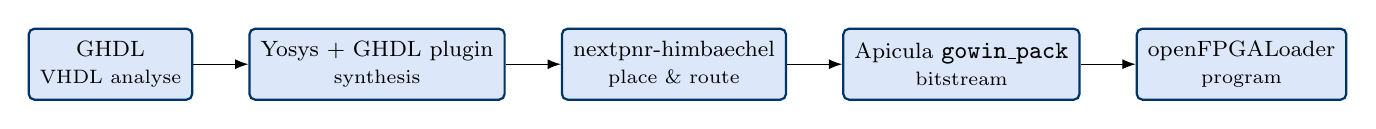
\begin{tikzpicture}[
  >=Latex, node distance=7mm,
  t/.style={draw=docblue, thick, rounded corners=2pt, fill=statefill,
            align=center, minimum height=9mm, font=\footnotesize, inner sep=4pt}]
\node[t] (ghdl) {GHDL\\\scriptsize VHDL analyse};
\node[t, right=of ghdl] (yosys) {Yosys + GHDL plugin\\\scriptsize synthesis};
\node[t, right=of yosys] (pnr) {nextpnr-himbaechel\\\scriptsize place \& route};
\node[t, right=of pnr] (pack) {Apicula \code{gowin\_pack}\\\scriptsize bitstream};
\node[t, right=of pack] (load) {openFPGALoader\\\scriptsize program};
\draw[->] (ghdl)--(yosys); \draw[->] (yosys)--(pnr);
\draw[->] (pnr)--(pack); \draw[->] (pack)--(load);
\end{tikzpicture}
\end{center}

\choice{Fully-open, Nix-pinned build}{%
The flake pins the exact tool versions and, where available, uses the
nixpkgs-matched Yosys GHDL plugin so the VHDL of NEORV32 and the Verilog of the
accelerator synthesise together. The result is a build that is reproducible on
any machine and free of proprietary tooling, at the cost of navigating the sharp
edges of a bleeding-edge open flow --- several of which became project
challenges.}

% ------------------------------------------------------------
\section{Verification Architecture}
Correctness is established in four layers, each checking the layer below against
the golden model, so that a failure is localised to one interface.

\renewcommand{\arraystretch}{1.3}
\begin{center}
\begin{tabular}{C{0.7cm} L{4.2cm} L{9.0cm}}
\thd{L} & \thd{Layer} & \thd{What it proves}\\
\trow 1 & Python golden model & Matches NIST Known-Answer Tests\\
2 & RTL vs.\ model (iverilog) & Each generated module matches the model on 25 vectors\\
\trow 3 & C driver vs.\ transport & The driver's register protocol is correct against an emulated peripheral\\
4 & End-to-end co-sim & The Wishbone adapter, driven exactly as NEORV32's XBUS does, carries the full AEAD protocol correctly\\
\end{tabular}
\end{center}
\renewcommand{\arraystretch}{1}

The whole suite (119 tests) runs from a clean checkout and is reproduced by
\code{nix flake check}. Layer~4 in particular replays the driver's real register
ordering through the bus adapter with a NEORV32-faithful pulsed-strobe master ---
the regression guard for the on-chip bus behaviour.

\warn{Simulation can only prove what it models. The co-simulation faithfully
reproduces the XBUS handshake and the driver protocol, but the final evidence of
correctness is the on-silicon run reported in the Project Report, where every case
was checked on-chip against the software reference.}

% ------------------------------------------------------------
\section{Design Choices Summary}
\renewcommand{\arraystretch}{1.3}
\begin{center}
\begin{tabular}{L{4.6cm} L{9.0cm}}
\thd{Decision} & \thd{Rationale}\\
\trow Model-first generation & One source of truth for RTL and reference; parameterisable\\
1 round / cycle permutation & Smallest crypto core; fits the GW2AR-18\\
\trow Layered engine (stream $\to$ MMIO $\to$ WB) & Each layer independently verifiable; clean interfaces\\
XBUS peripheral & Loose coupling; no CPU pipeline changes\\
\trow MMIO-word data plane & Simple, no DMA; accepts data-movement overhead\\
Drop M extension & Unused by \code{rv32i} firmware; frees area to fit\\
\trow Bounded 32-byte payloads & Fits small on-chip buffers; streaming is future work\\
Fully-open Nix toolchain & Reproducible; no vendor lock-in\\
\end{tabular}
\end{center}
\renewcommand{\arraystretch}{1}

% ------------------------------------------------------------
\section{Known Limitations}
\begin{itemize}
\item Payloads are bounded to 32 bytes of associated data and 32 bytes of message
      per call; arbitrary-length rate-block streaming is the natural extension.
\item The memory-mapped, word-at-a-time data plane dominates latency for larger
      payloads; a DMA or wider datapath would improve throughput.
\item Only the AEAD128 mode is exercised on hardware; hash/XOF modes exist in the
      model but are not integrated on-board.
\item No side-channel or constant-time characterisation has been performed; this
      is a functional and performance design, not a hardened one.
\end{itemize}

\vfill
\begin{center}\small\color{gray}
Design Document --- companion to the RASD and the Project Report.
\end{center}

\end{document}
